\sectionframe{Modeling of logical expressions}
\begin{frame}
 \frametitle{Example: Adventure Inc.}
 \begin{figure}
  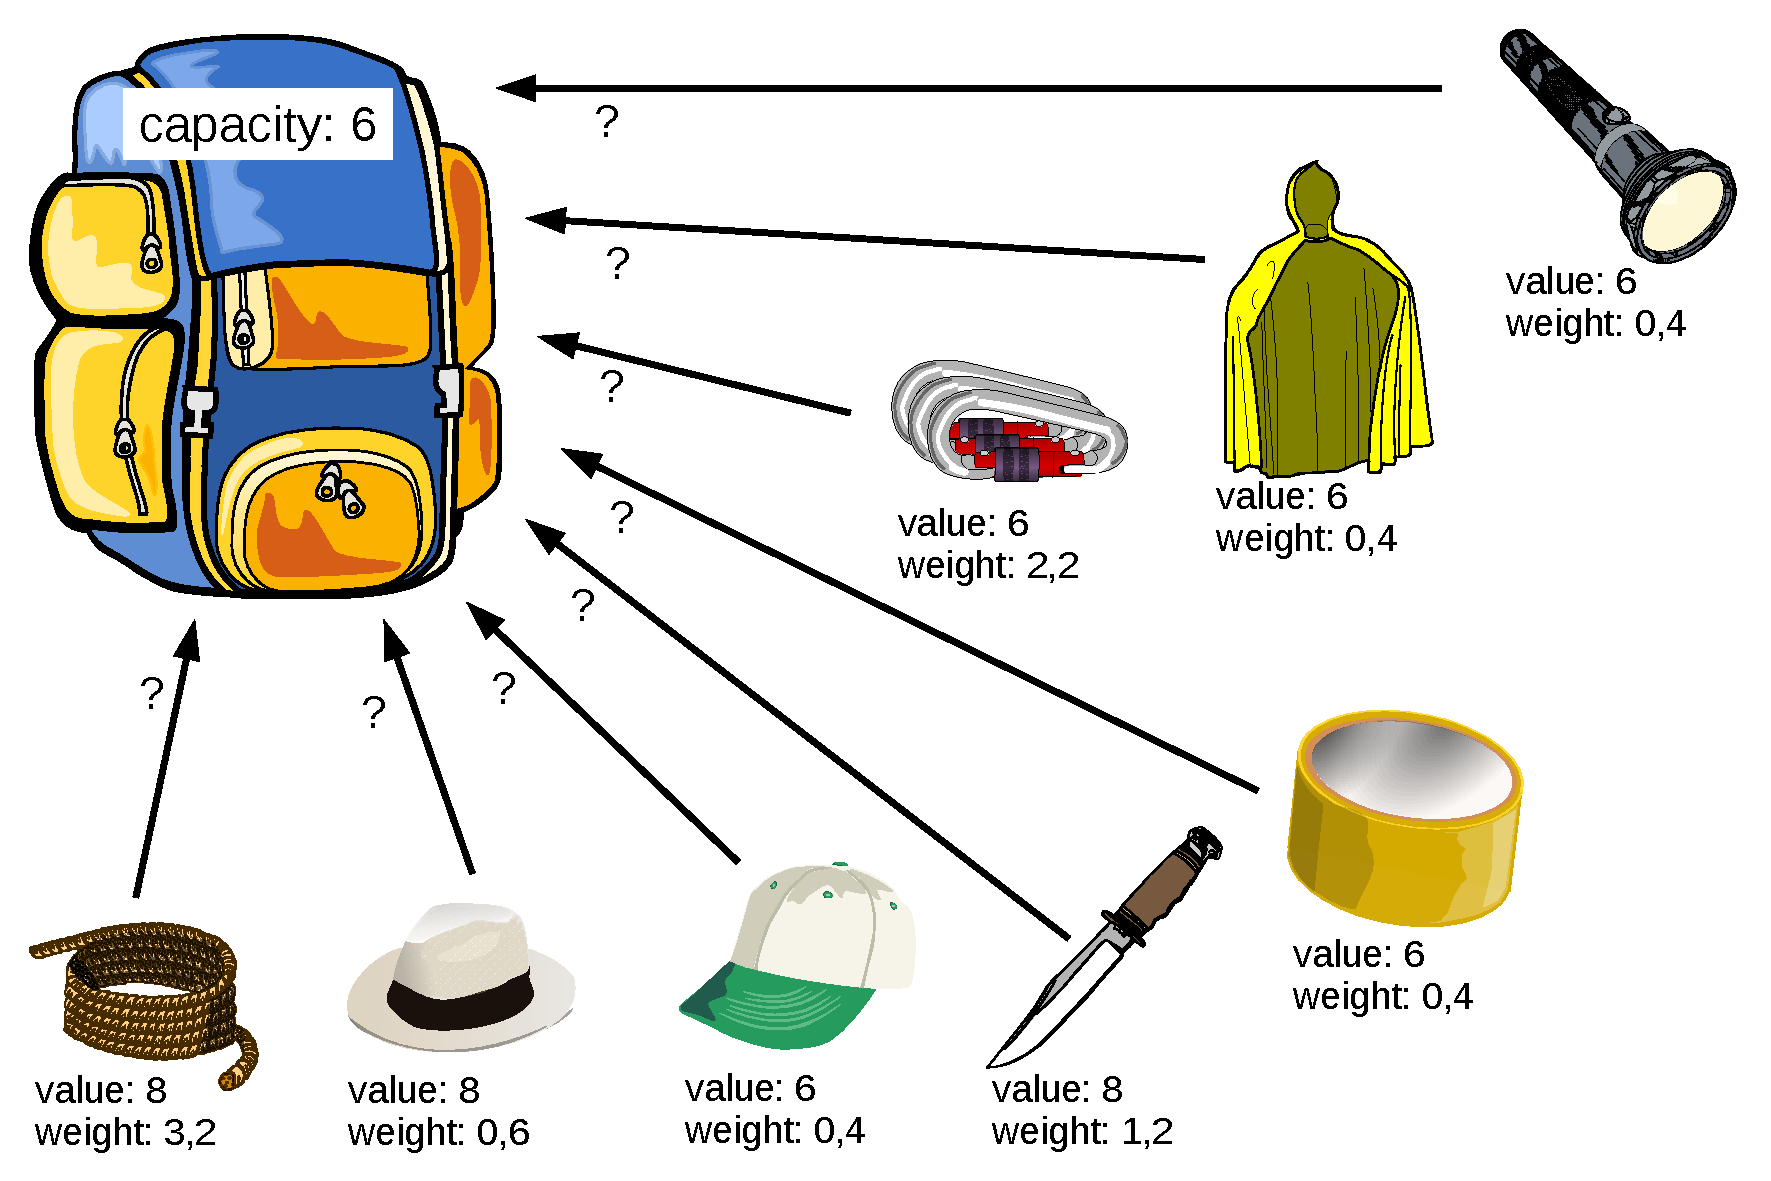
\includegraphics[width=\linewidth]{Bilder/Rucksackproblem}
 \end{figure}
\end{frame}

\begin{frame}\small
 \frametitle{Model: Knapsack problem}
 \begin{tabularx}{\linewidth}{lL}
  \multicolumn{2}{l}{\textbf{Index sets}:}\\
    $I$ & Set of items\\
  \multicolumn{2}{l}{\textbf{Parameters}:}\\
    $w_i$ & weight of item~$i\in I$\\
    $u_i$ & value of item~$i\in I$\\
    $c$ & capactiy of the knapsack\\
  \multicolumn{2}{l}{\textbf{Decision variables}:}\\
    $x_i$ & binary decision variable; indicates if item~$i\in I$ is packed\\[1ex]
  \multicolumn{2}{l}{\textbf{Model description}:}\\[1ex]
  \multicolumn{2}{l}{
	$
	\begin{array}{rllr}
	  \max & \displaystyle\sum_{i\in I} u_i\cdot x_i & & \\[3ex]
	  s.t. & \displaystyle\sum_{i\in I} w_i\cdot x_i \leq c & & \mathrm{(I)}\\
		  & \alert{x_i \in \{0,1\}} & \quad\forall i\in I & \\
	\end{array}
	$ 
  }\\[1ex]
 \end{tabularx}
\end{frame}

\begin{frame}
 \frametitle{Logical operators}
 \begin{description}
 \item[$\neg$] logical \textbf{{negation}}  
 \item[$\wedge$] logical \textbf{{and}}
 \item[$\vee$] logical \textbf{{or}}
 \item[$\veebar$] logical \textbf{exklusive or} (``xor'')
 \item[$\Rightarrow$] logical \textbf{{implication}}
 \item[$\Leftrightarrow$] logical \textbf{{equivalence}}
\end{description}
\begin{block}{Truth table in numerical representation}
 \centering\footnotesize
 \begin{tabular}{*{9}{c}}
  \toprule
  $A$ & $B$ & $\neg A$ & $\neg B$ & $A\wedge B$ & $A\vee B$ & $A \veebar B$ & $A\Rightarrow B$ & $A\Leftrightarrow B$\\
  \midrule
  1 & 1 & 0 & 0 & 1 & 1 & 0 & 1 & 1\\
  1 & 0 & 0 & 1 & 0 & 1 & 1 & 0 & 0\\
  0 & 1 & 1 & 0 & 0 & 1 & 1 & 1 & 0\\
  0 & 0 & 1 & 1 & 0 & 0 & 0 & 1 & 1\\
  \bottomrule
 \end{tabular}
\end{block}
\end{frame}

\begin{frame}
 \frametitle{Logical operators in binary optimization models}
 {\small Example: Let $x_1$ and $x_2$  be binary decision variables of a knapsack problem, representing items $I_1$ and $I_2$.}
 \begin{center}\footnotesize
\begin{description}
  \only<1>{\item[$\neg I_1$:] Get the value of $I_1$ not being packed.
  \begin{itemize}\item$
    1-x_1
  $\end{itemize}}
  \only<1>{\item[$I_1\wedge I_2$:]  Both $I_1$ and $I_2$ must be packed.
  \begin{itemize}\item$
    x_1+x_2 = 2
  $\end{itemize}}
  \only<1>{\item[$I_1\vee I_2$:]  At least one of the items has to be packed.
  \begin{itemize}\item$
    x_1+x_2 \geq 1
  $\end{itemize}}
  \only<1>{\item[$\neg(I_1\wedge I_2)$:] At most one of the items may be packed.
  \begin{itemize}\item$
    x_1+x_2 \leq 1
  $\end{itemize}}
  \only<2>{\item[$\neg(I_1\vee I_2)$:]  None of the items may be packed. 
  \begin{itemize}\item$
    x_1+x_2 = 0
  $\end{itemize}}
  \only<2>{\item[$I_1\veebar I_2$:]  Exactly one of the items must be packed. 
  \begin{itemize}\item$
    x_1+x_2 = 1
  $\end{itemize}}
  \only<2>{\item[$I_1\Rightarrow I_2$:]  If $I_1$ is packed, $I_2$ must also be packed. 
  \begin{itemize}\item$
    x_1 \leq x_2
  $\end{itemize}}
  \only<2>{\item[$I_1\Leftrightarrow I_2$:]  The decision is identical for both items. 
  \begin{itemize}\item$
    x_1 = x_2
  $\end{itemize}}
\end{description}
 \end{center}
\end{frame}
